\begin{figure}[H]
  \begin{subfigure}[b]{.5\textwidth}
    \centering
    \includegraphics[width=.8\textwidth]{images/model\_m}
    \caption{Teclado IBM Model M (1984)}
  \end{subfigure} 
  \hfill
  \begin{subfigure}[b]{.5\textwidth}
    \centering
    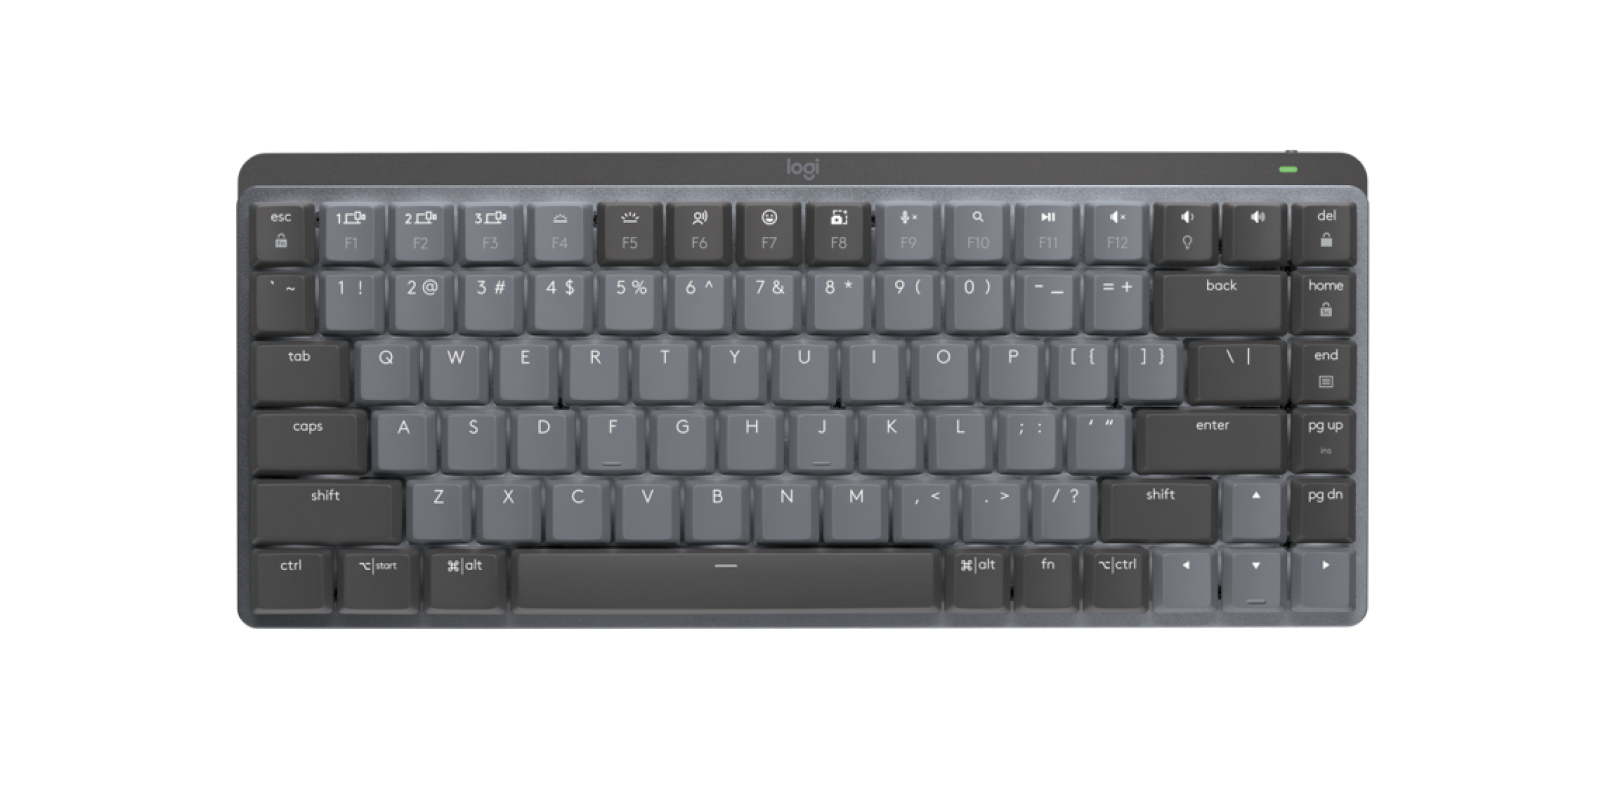
\includegraphics[width=\textwidth]{images/logitech}
    \caption{Teclado Logitech MX Mechanical (2022)}
  \end{subfigure}
  \caption{Comparativa teclado antiguo y actual}
\end{figure}

\image{android\_keyboard}{.4\textwidth}{Teclado en Android}

Como podemos ver, los teclados no han variado en los ultimos 40 años, ni siquiera para adaptarse a las pequeñas pantallas táctiles de los móviles.

\subsection{Diseño anticuado}
  \subsubsection{Forma del teclado}
  Quizás nunca nos lo hayamos preguntado puesto que tenemos muy interiorizada la forma de los teclados, pero si lo pensamos un poco, es peculiar la posición relativa de las teclas. Cada fila tiene un pequeño desfase con las demás en vez de estar alineadas. Esto es un legado de sus antecesoras, las máquinas de escribir, donde por limitaciones mecánicas esto tenía que ser así y evitar choques entres las piezas móviles de cada tecla.
  \image{typewriter}{.3\textwidth}{Detalle de las letras en una máquina de escribir}

  Este posicionamiento relativo de las teclas supone un problema a la hora de escribir, ya que la forma óptima de hacerlo sería la siguiente:
  \image{mechanography}{.3\textwidth}{``Mapa'' de mecanografía}
  
  Sin embargo, para escribir así, las muñecas terminan en posiciones un poco forzadas, y los dedos hacen movimientos incómodos. Para arreglar esto surgieron los teclados ortolineales, donde todas las filas están alineadas y los dedos se mueven en una línea recta. Estos teclados suelen tener todas las teclas del mismo tamaño, optimizando así la cantidad de teclas que podemos tener ocupando el mismo espacio (donde antes había una barra espaciadora pueden entrar varias teclas). Como se puede ver en la siguiente imagen, normalmente también prescinden del teclado numérico para reducir el tamaño, este modelo se conoce como ``75\%'' ya que tiene 75 teclas mientras que los teclados comunes (``100\%'') tienen 104/105 teclas. Otras variantes comunes son ``40\%'', ``60\%'', ``65\%'' 
  \image{ortholinear}{.3\textwidth}{Teclado ortolineal \textit{RGB75}}

  \subsubsection{Ubicación de las letras}
  Otro legado que nos dejaron las máquinas de escribir es la distribución QWERTY, que probablemente sea la única distribución que hemos visto a lo largo de nuestra vida. El problema con esta disposición es que, si bien distribuye las letras de forma que se usan las dos manos por igual, se diseñó en la decada de 1860, por lo que uno de sus objetivos era el de reducir los atascos en las máquinas de escribir separando las teclas más usadas de la parte central. 

  En contra, ahora que gracias a la electrónica no tenemos estas limitaciones, se han diseñado distribuciones que minimizan la distancia media que se debe recorrer al escribir, por lo que una vez acostumbrados a ellas se puede escribir más rápido y reduciendo la fatiga en los dedos. Las dos más extendidas son DVORAK y COLEMAK. 
  \image{qwerty}{.3\textwidth}{Distribución QWERTY}
  \begin{figure}[H]
    \begin{subfigure}[b]{.5\textwidth}
      \centering
      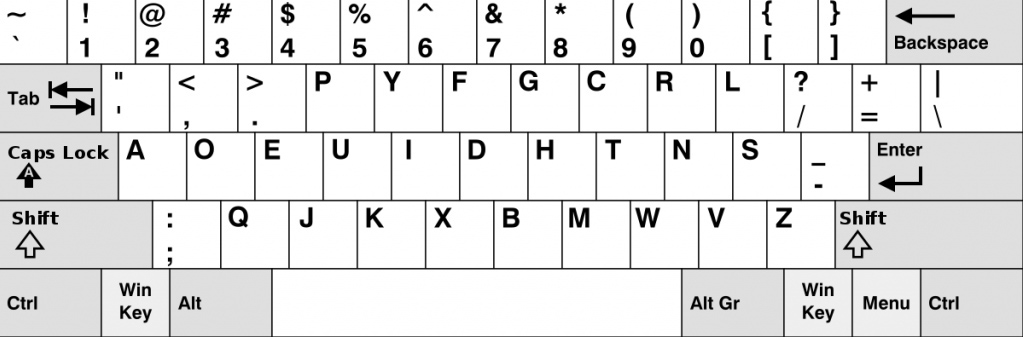
\includegraphics[width=.6\textwidth]{images/dvorak}
      \caption{Dvorak}
    \end{subfigure} 
    \hfill
    \begin{subfigure}[b]{.5\textwidth}
      \centering
      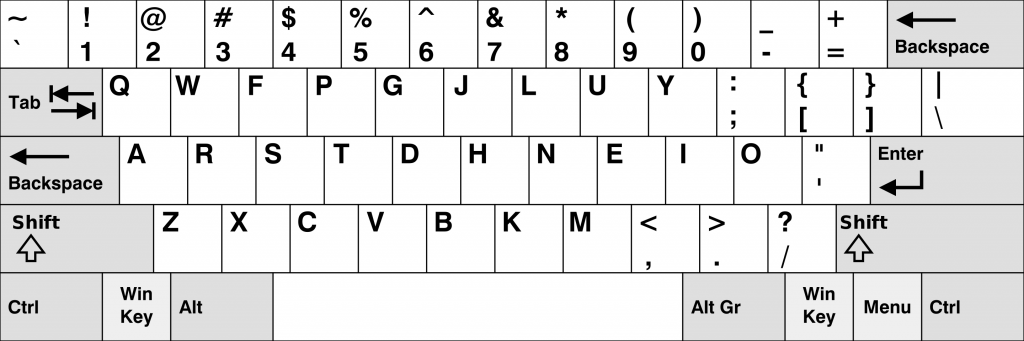
\includegraphics[width=.6\textwidth]{images/colemak}
      \caption{Colemak}
    \end{subfigure}
    \caption{Distribuciones alternativas}
  \end{figure}

\subsection{Ergonomía}
Gracias a la apasionada y extensa comunidad de aficionados a los teclados mecánicos, en los últimos años han aparecido multitud de diseños que incorporan diferentes cambios respecto al paradigma actual.\newline

Como hemos comentado ya, uno de los problemas más comunes en gente que usa mucho los teclados es la aparicion de dolencias en las muñecas, a fin de que estas se posicionen de una forma más natural y cómoda, se opta por partir el teclado en dos mitades, lo que se conoce como teclados \textit{split}.
\image{quefrency}{.45\textwidth}{Teclado \textit{Quefrency}}

Otra técnica, mayormente usada en teclados \textit{split}, consiste en levantar la parte central del teclado, de forma que la mano quede en una posición más natural en vez de estar paralela al plano que forma la mesa. Lo mejor de esta mejora es que se puede añadir a cualquier teclado añadiendo algún objeto para levantarlo.
\image{dygma}{.3\textwidth}{Teclado \textit{Dygma Raise}}

Otros diseñadores integran reposamuñecas de una forma más eficaz y cómoda que la típica ``rampa'' de plástico que estamos acostumbrados a ver.
\image{moonlander}{.3\textwidth}{Teclado \textit{Moonlander}}

Muchos teclados dotan de una mayor utilidad a los pulgares, que normalmente solo utilizamos para la barra espaciadora, añadiendo unas cuantas teclas en lo que comunmente se conoce como \textit{thumb cluster}.
\image{ergodox}{.4\textwidth}{Teclado \textit{Ergodox}}

El mayor ejemplo de estas ideas es el \textit{Dactyl Manuform}, un teclado que debido a su particular forma ni siquiera puede funcionar con una PCB y tiene que soldarse a mano la unión entre todos sus componentes. El beneficio de su diseño es que tiene en cuenta la forma de las manos, por lo que las teclas se encuentra posicionadas acorde al movimiento de los dedos. Además, hay usuarios que optan por modificar el diseño e integrarle una \textit{trackball} para poder controlar el cursor sin tener que mover la mano entre el teclado y el ratón.
\image{manuform}{.3\textwidth}{Teclado \textit{Dactyl Manuform} con trackball}\label{img:dactyl}

\vspace*{\fill}
\hr
En esta web\cite{paper} se pueden ver varios estudios sobre la relación entre el diseño del teclado y sus efectos en la salud
